%%%%%%
% Final plots from results



\begin{figure}[H]
\centering
\begin{minipage}[b]{.66\linewidth}
	\centering
	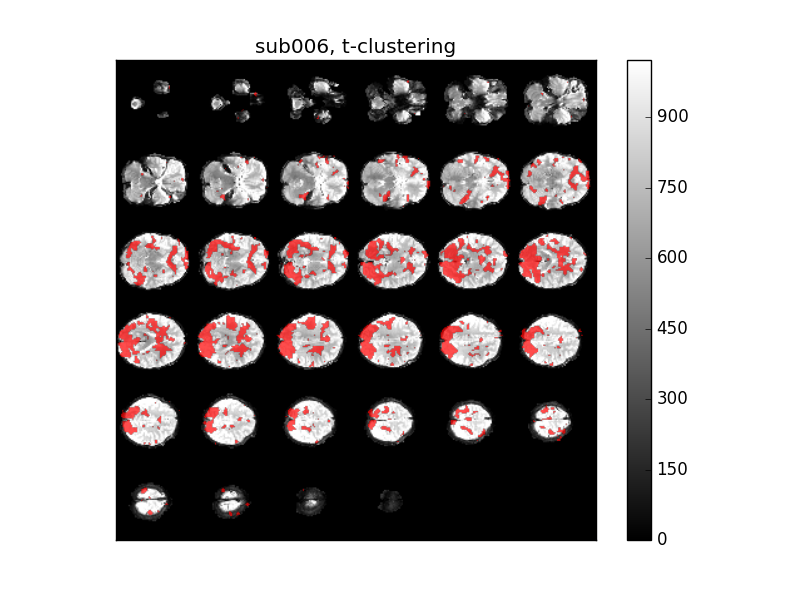
\includegraphics[width=.8\linewidth]{../images/sub006_t_overlay.png} 
	\caption{Quantile-based clustering for Subject 6's t-statistics. 
	(Blue areas denote significant regions)}
	\label{fig:clustert}
\end{minipage}	

\begin{minipage}[b]{.66\linewidth}
	\centering
		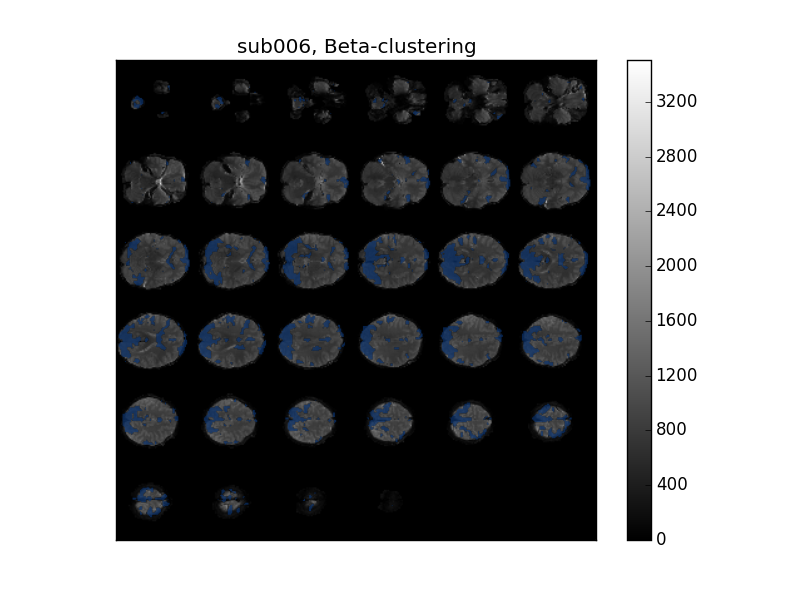
\includegraphics[width=.8\linewidth]{../images/sub006_beta_overlay.png} 
	\caption{Quantile-based clustering for Subject 6's $\hat{\beta}$ coefficients. 
	(Blue areas denote significant regions)}
	\label{fig:clusterbeta}
\end{minipage}

\begin{minipage}[b]{.66\linewidth}
	\centering
		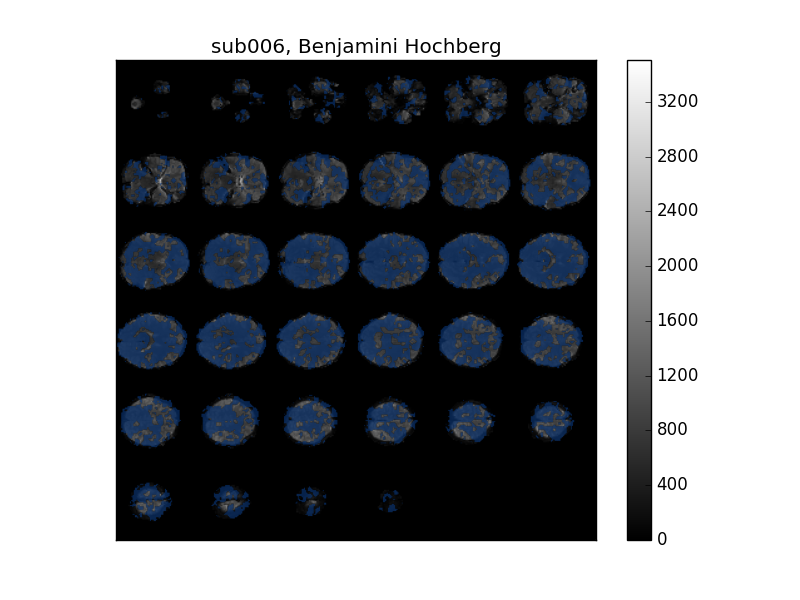
\includegraphics[width=.8\linewidth]{../images/sub006_bh_overlay.png} 
	\caption{Benjamini-Hochberg clustering for Subject 6. 
	(Blue areas denote significant regions)}
	\label{fig:clusterBH}
\end{minipage}
\end{figure}


\begin{figure}[H]
\centering
\begin{minipage}[b]{.66\linewidth}
	\centering
	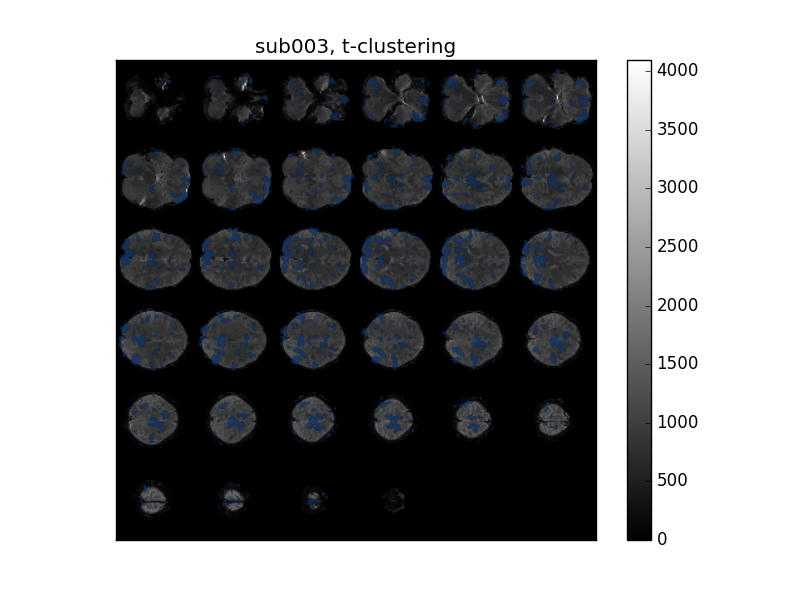
\includegraphics[width=.8\linewidth]{../images/sub003_t_overlay.png} 
	\caption{Quantile-based clustering for Subject 3's t-statistics. 
	(Blue areas denote significant regions)}
	\label{fig:clustersub3}
\end{minipage}	

\begin{minipage}[b]{.66\linewidth}
	\centering
		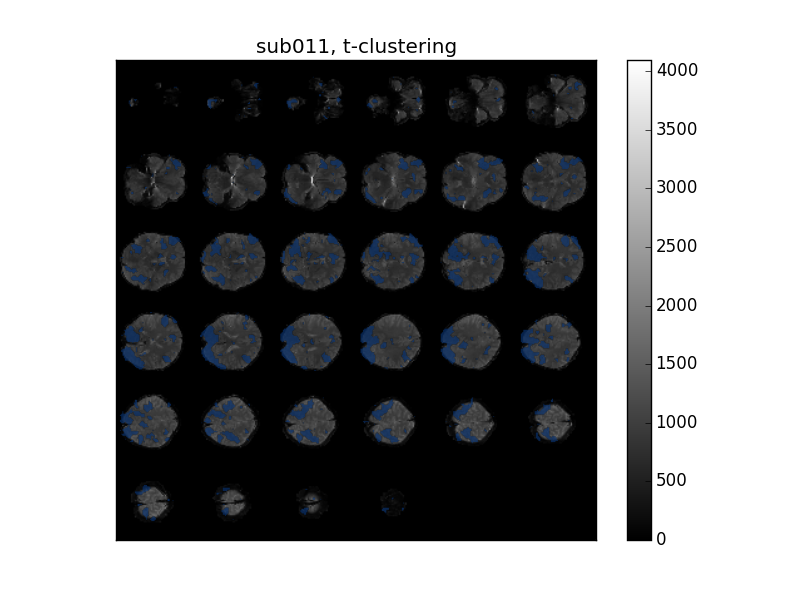
\includegraphics[width=.8\linewidth]{../images/sub011_t_overlay.png} 
	\caption{Quantile-based clustering for Subject 11's t-statistics. 
	(Blue areas denote significant regions)}
	\label{fig:clustersub11}
\end{minipage}

\begin{minipage}[b]{0.66\linewidth}
	\centering
		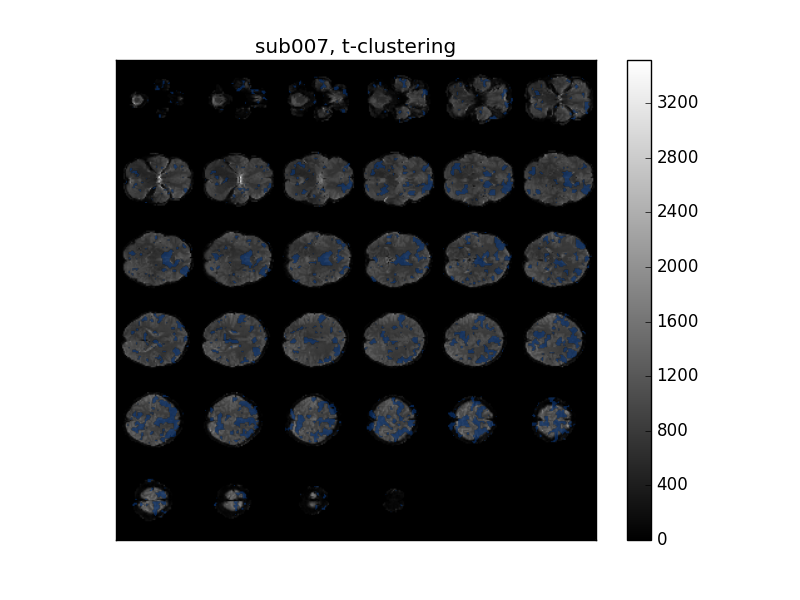
\includegraphics[width=.8\linewidth]{../images/sub007_t_overlay.png} 
	\caption{Quantile-based clustering for Subject 7's t-statistics. (Blue areas denote significant regions)}
	\label{fig:clustersub7}
\end{minipage}
\end{figure}




